\documentclass[10pt,]{beamer}
\usepackage[utf8]{inputenc}
\usepackage[spanish]{babel}
\usepackage{graphicx}
%\usepackage[round]{natbib}

% Este archivo corresponde a los paquete y combinaciónes de colores necesarias para dejarlo con los colores azules de la UCM
% Plantilla realizada por Carlos Palacios junio de 2015
\usepackage{amsmath}
\usepackage{amsfonts}
\usepackage{amssymb}
\usetheme{CambridgeUS}

\usepackage{xcolor}

\setbeamercolor{normal text}		{fg=black,bg=white} %color del texto normal
\setbeamercolor{alerted text}		{fg=blue}
\setbeamercolor{example text}		{fg=black}
\setbeamercolor{background canvas}  {fg=pink, bg=white}%diapositiva de fondo blanco
\setbeamercolor{background}         {fg=green, bg=yellow}
\setbeamercolor{frametitle}			{fg=blue!60!black,bg=gray!10}%color del texto del título y su fondo
\setbeamercolor{title}				{fg=yellow!10!white,bg=blue!60!black}%color del texto del título y su fondo, solo para la lámina de título
\setbeamercolor{palette primary}    {fg=blue!60!black, bg=gray!30!white}%colores de las distintas paletas
\setbeamercolor{palette secondary}  {fg=blue!70!black, bg=gray!20!white}%colores de las distintas paletas
\setbeamercolor{palette tertiary}   {fg=white, bg=blue!60!black}%colores de las distintas paletas
\setbeamercolor{block title}{bg=blue!60!black,fg=white}%color del título de un bloque
%\setbeamercolor{block body}{fg=black,bg=gray!10}

%\setbeamercolor{author in head/foot}{bg=blue}
%\setbeamercolor{section in head/foot}{fg=yellow}

\setbeamercolor{author in title}{fg=blue}
\setbeamercovered{transparent=10}

\usepackage{hyperref}


\author[Nombre corto]{Nombre alumno \\ \tiny correo u otro}
\title[Titulo corto]{Título del proyecto de titulación}
\subtitle{Exámen de titulación}
\institute[ICO - UCM]{Escuela de Ingeniería en Construcción\\Universidad Católica del Maule}
\date[]{\today}


% El siguiente código es para generar índice por cada sección, ver pdf.
% \AtBeginSection[]
% {
% 	\begin{frame}{Contenido}2% \tableofcontents[currentsection]
% 	\end{frame}
% }


\begin{document}

	\logo{
\includegraphics[scale=0.15]{imagenes/logoUniversidad}}
\begin{frame}[plain]

\begin{columns}

	\begin{column}{5cm}
	
\includegraphics[scale=0.2]{imagenes/logoICO}
	\end{column}

	\begin{column}{5cm}
	\begin{flushright}
	
\includegraphics[scale=0.3]{imagenes/logoUCM}
	\end{flushright}
	\end{column}

\end{columns}
\maketitle

\end{frame}
%%-------------------------------------------------------------------------------------

 \begin{frame}{Contenido}
 \tableofcontents
 \end{frame}

%%-------------------------------------------------------------------------------------

\section{Título de la sección}

	\begin{frame}{Título de la diapositiva}
		Agregar texto...
	\end{frame}

	\begin{frame}{Título segunda lámina}{Se puede agregar un subtítulo si es requerido}
		Agregar texto...		
	\end{frame}


\section{Título de la segunda sección}

	\begin{frame}{Título de la tercera diapositiva}
		\begin{block}{Objetivos}
			\begin{enumerate}
				\item<1-> Objetivo 1 %El <> y el 1- significa que se mostrará de la lámina 1 en adelante 
				\item<2-> Objetivo 2 %Otra opción sería <1> y solo se mostraría en la lámina 1
				\item<3-> Objetivo 3 %Otra opción más, es <1-2> solo se mostrará en la lámina 1 y 2
			\end{enumerate} 
		\end{block}
	\end{frame}

% Otro ejemplo de lamina
	\begin{frame}{Componentes del hormigón}{Agua}
		\begin{description}
			\item[Agua]El  agua  para  el  uso  de  hormigones  debe  cumplir  con  la  Norma  NCh1498.  El  agua  potable  						cumple con  estas exigencias  \cite{solminihac2008}.
		\end{description}
	
		\begin{center}
			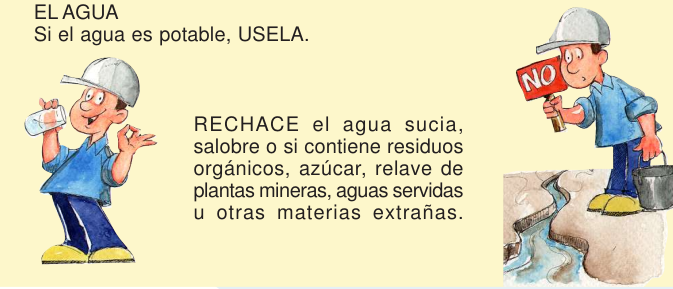
\includegraphics[width=0.85\linewidth]{imagenes/agua} 
		\end{center}
	\end{frame}


\section{Bibliografía}
	
	\begin{frame}{Bibliografía}
		\bibliographystyle{apalike}
		\bibliography{perifericos/bibliografia}
	\end{frame}


\end{document}